\documentclass[11pt,a4paper]{article}
\usepackage[margin=22mm]{geometry}
\usepackage{amsmath,booktabs,graphicx,hyperref}
\title{M4 geometry and bias study in the 180 nm CSA}
\author{NAUSICAA calculation record}\date{\today}
\begin{document}\maketitle
The M4 width and length are multiplied by 2, 4, 8 and 16, retaining $W/L=2$.
The first scan retains the original gate bias, 0.62 V. The second adjusts this
bias for factors 2, 4 and 8 to recover the original quiescent output voltage
to within 10 microvolts. All other transistor dimensions and bias voltages,
including the feedback transistor, remain as supplied.

The external input capacitance is 1.25 pF, the feedback capacitor is 3 fF,
the supply is 1.8 V and the temperature is 20 degrees Celsius. The supplied
NOIMOD=2 card is used throughout. Intrinsic MOS capacitances are included.
Noise is stationary about the zero-signal operating point, integrated from
0.1 Hz to 1 MHz. These are schematic-level calculations with the supplied
process card; layout parasitics and process corners remain to be evaluated.

The input is the uniform mean arrival distribution over 10 ms. Each ion
follows the finite 5 mm approach at 3 m/s to a central 0.5 mm square pad in an
infinite grounded plane. Its induced charge is $e\Delta\phi_w$, without
renormalization. The estimator uses centered 300 microsecond averages at the
frame boundaries and $\alpha=\exp(-10\,\mathrm{ms}/0.3\,\mathrm{s})$.
The signal gain is calibrated from the simulated waveform of one ion.

\section*{Frame charge and operating point}
\begin{center}\begin{tabular}{rrrrrr}\toprule
$W$ & $L$ & Gate & ENC & Gain & Output DC\\
($\mu$m) & ($\mu$m) & (V) & (electrons RMS) & ($\mu$V/ion) & (V)\\\midrule
0.72 & 0.36 & 0.620000 & 295.9 & 15.47 & 0.879 \\
1.44 & 0.72 & 0.620000 & 133.7 & 0.27 & 0.126 \\
1.44 & 0.72 & 0.585809 & 172.0 & 21.57 & 0.879 \\
2.88 & 1.44 & 0.620000 & 126.9 & 0.20 & 0.115 \\
2.88 & 1.44 & 0.556803 & 137.9 & 26.54 & 0.879 \\
5.76 & 2.88 & 0.620000 & 126.5 & 0.19 & 0.112 \\
5.76 & 2.88 & 0.541323 & 129.7 & 32.65 & 0.879 \\
11.52 & 5.76 & 0.620000 & 126.4 & 0.18 & 0.111 \\
\bottomrule\end{tabular}\end{center}
The fixed-bias scan changes both noise and operating point. Comparing gain
alongside ENC identifies this change. The adjusted-bias variants restore
the output level before their signal and noise are evaluated.
\begin{center}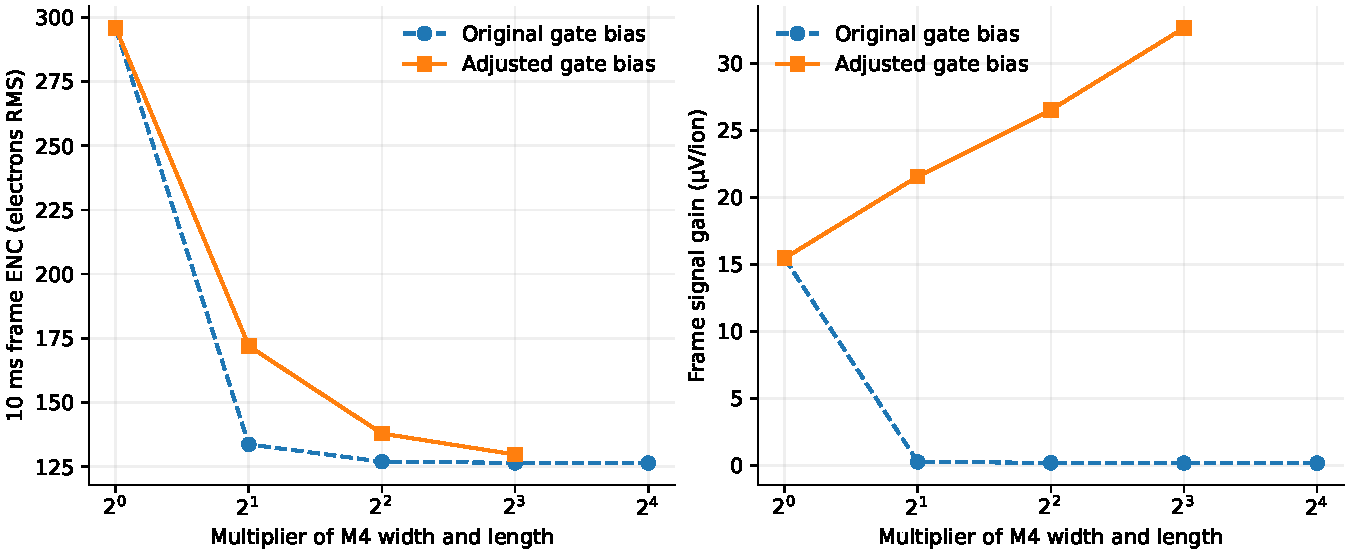
\includegraphics[width=\linewidth]{enc_and_gain.pdf}\end{center}

\section*{Injection, speed, power and linearity}
The injection pulse has a 1 microsecond plateau and 10 ns edges, with total
charge $e$. Its ENC uses a trapezoidal filter with rise and flat-top durations
of 300 microseconds, evaluated at the noiseless-template peak.
Rise time is the 10--90 percent interval relative to the unfiltered peak.
The gain ratio compares the uniform 1000-ion response with 1000 times the
one-ion response. Supply power is the DC value at 1.8 V.
Rows after the original use the adjusted gate bias.
\begin{center}\begin{tabular}{rrrrr}\toprule
Dimension multiplier & Injection ENC & Rise & Power & Gain ratio\\
 & (electrons RMS) & ($\mu$s) & ($\mu$W) & (1000 ions)\\\midrule
1 & 203.6 & 3.19 & 343.52 & 0.99784 \\
2 & 114.8 & 4.27 & 343.52 & 0.99839 \\
4 & 89.5 & 5.22 & 343.52 & 0.99881 \\
8 & 83.3 & 6.46 & 343.52 & 0.99914 \\
\bottomrule\end{tabular}\end{center}
\begin{center}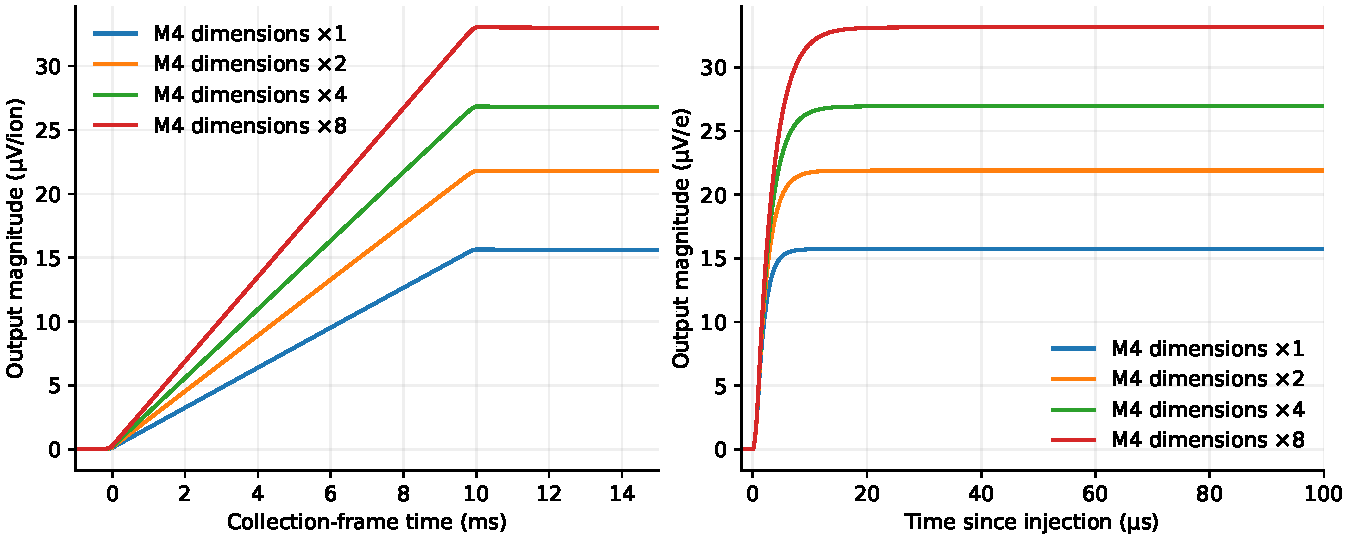
\includegraphics[width=\linewidth]{responses.pdf}\end{center}

The selected adjusted variant (dimension multiplier 8) reaches $S/N>5$ at 649 ions; adjacent integer counts are verified at both timestep resolutions.
\section*{Numerical checks and reproduction}
The original geometry reproduces the preceding ENC calculation within a
relative tolerance of $10^{-9}$. The analysis checks input charge, halves
the transient timestep, doubles noise sampling from 200 to 400 points per
decade, changes quadrature order from 8 to 16 and halves the injection
peak-search timestep. Signal and spectral differences are below $10^{-3}$;
quadrature differences are below $10^{-5}$ and charge errors below $2\times10^{-5}$.
Integrated device noise variances reproduce the total within $10^{-3}$.
The 1000-ion signal is checked at both transient resolutions.

Raw data, operating points, spectra, source hashes and logs are in
\texttt{results/ltspice/m4\_scan/raw.h5}. Julia writes the reduced numerical
results to \texttt{analysis.h5}. The original received circuit is preserved.
Derived circuit decks include the selected geometry and gate voltage.
The accompanying README gives the commands for acquisition, bias adjustment,
analysis and report generation.
\end{document}
